% !TeX spellcheck = cs_CZ

\documentclass[a4paper]{article}
\usepackage[english]{babel}
\usepackage[utf8x]{inputenc}
\usepackage[T1]{fontenc}
\usepackage{listings}
\usepackage[a4paper,margin=2cm]{geometry}
\usepackage{amsmath}
\usepackage{graphicx}
\usepackage[colorinlistoftodos]{todonotes}
\usepackage[colorlinks=true, allcolors=blue]{hyperref}
\usepackage{wasysym} % smileys
\usepackage{fancyhdr}
\setlength\parindent{0pt} % indent

% my commands:
\newcommand{\n}{\newline}
\newcommand{\tab}{\hspace{1cm}}

\begin{document}

\title{Ptakopět \\ \large Překlad tam a kontrolně zpět }
\author{Vilém Zouhar}
\date{December 2018 \\ Rev. 3}
\maketitle 

% https://www.cs.uic.edu/~jbell/CourseNotes/OO_SoftwareEngineering/SE_Project_Report_Template.pdf

\section{Overview}
Ptakopět (Překlad Tam A KOntrolně zPĚT) is an agile browser agnostic plugin, which aims to help people translate to languages, where they are unable to verify the quality of the translation, by offering backward translation of the result. The issue at hand is sometimes known as \textit{Outbound Translation}, which is a complement to \textit{Gisting}. Both in \textit{Gisting} and \textit{Outobound Translation}, the user speaks only one of the languages. In the former, the users is responsible for creating correct messages, while in the later the responsibility is to correctly interpret them. 

\subsection{The purpose of the project}
Many users use machine translation to verify their own translation, or can at least affirm, that the machine translation is valid. Translation systems are, however, not perfect and despite their great power, they tend to perform poorly on unseen phenomena (unknown words, unexpected word order, etc.). Users translating to languages, which they don't master enough to validate the translation could use Ptakopět to verify (and assure them), that the machine translation output is valid. Due to the fact that many encounters with foreign languages happen on the Internet, Ptakopět is developed as a browser extension.

\subsection{Other solutions}
Backwards translation is only one of the solutions to \textit{Outbound Translation}. One of the possible solutions could include more autonomous systems, such as text highlighting or numeric responses. Backward translation relies on the ability of the user to assess the differences between texts.

\subsection{The scope}
Ptakopět aims to provide a backward translation interface to already existing translation engines. It does not do the translation itself in any way. Existing translation backends are provided by the Charles University, namely by Martin Popel and other associates (as of version 1.0.4, CS-EN and EN-FR language pairs are available). The interface is provided in a form of browser agnostic plugin, that can also be hardwired to website as a plain script.

\vspace{1cm}
\begin{center}
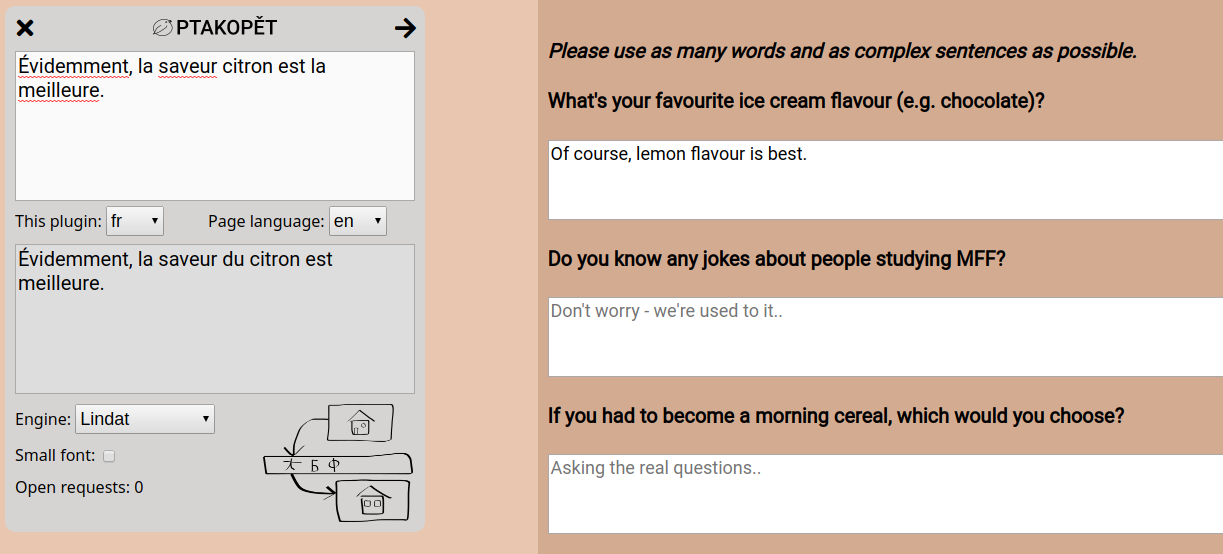
\includegraphics[width=\textwidth]{screenshot_3}
\end{center}

\section{Implementation}
The plugin itself is written in JavaScript, but injects HTML, CSS and jQuery framework into web page. Making the plugin indifferent to whether it is run as a background sciprt (browser plugin) or as an user script (included in web page) posed a substantial obstacle. Resulting implementation works, but is unfortunately affected by web styling. Eg.  website CSS can define the looks of the plugin, which is not intended and can result in usable, but not aesthetically pleasing design. \\
Ptakopět tries to capture all input events to \textit{textareas} and \textit{inputs}. This is a very robust approach, but about half of the websites (as of 2018) use custom input elements (to provide styling and extra functionaliy). As a result, these elements can't be captured using Ptakopět. This is obviously a radical usability issue, but we didn't find any universal solution to this problem. \\
Text events are processed and forwarded to translation engine using AJAX requests. This could eventually pose a threat to these backends should the plugin be used by many people simultaneously. The engines would be glutted by requests, as every keypress invokes one or two translations. They are indistinguishable from legit requests, as the plugin works user-side. This could be solved by a standard approach of postponing requests to some interval of no key press (\textit{ptakopet\_arch.js:89}).

\subsection{Technical details}
The code itself is located in the \textit{src/} directory. The \textit{manifest.json} file is obligatory for all plugin versions. When Ptakopět is run as a background script (browser plugin), then \textit{ptakopet\_background\_bootstrap.js} is executed, which adds listeners to context menu and icons. Then \textit{ptakopet\_init.js} is run as a user script and from this point on, it is identical to having the script run from the web page. Due to asynchronous loading, the startup functions are called in \textit{ptakopet\_init\_user.js}. Generally, \textit{ptakopet\_init.js} handles visual elements (eg. displaying \textit{floater.html}, CSS etc.), while \textit{ptakopet\_translator.js} takes care of the translation flow. Ptakopět was designed to support fast addition of new translator backends or supported languages. Each translation object in Ptakopět manages it's own AJAX requests in a standardized form.

\vspace{1cm}
\begin{center}
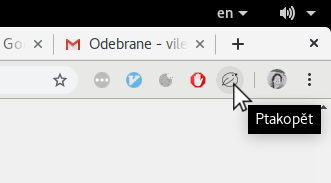
\includegraphics[width=0.4\textwidth]{screenshot_5}
\hspace{2cm}
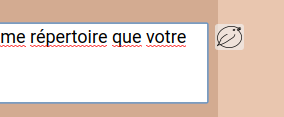
\includegraphics[width=0.4\textwidth]{screenshot_6}
\end{center}

\section{Standalone instalation}
This plugin can be also hardwired into a web page (mostly for presentation purposes). It is sufficient to download all source files (the \textit{src/} directory on GitHub) and add this line to your target HTML file: \begin{lstlisting}
<script id='ptakopet_init' src='dev/ptakopet/js/ptakopet_init.js'></script>
\end{lstlisting}


\section{Browser plugins}
Basic demonstration and info about Ptakopět online publication is located at \href{http://ptakopet.vilda.net}{ptakopet.vilda.net}. Ptakopět was also presented at MFF Open Days (November 2018). The presentation page is located at \href{https://vilda.net/s/dod\_ptakopet}{vilda.net/s/dod\_ptakopet}. The plugin itself is distributed as a \href{https://chrome.google.com/webstore/detail/ptakop\%C4\%9Bt/hgjlgmhmcmcmjiclegnipnaeejpibjmn}{Chrome} and \href{https://addons.mozilla.org/en-US/firefox/addon/ptakop\%C4\%9Bt/}{Firefox} extension. The plugin was also submitted to the Opera addon store, but still hasn't been reviewed.
Source code is published at a GitHub repository:\\ \href{https://github.com/zouharvi/ptakopet}{github.com/zouharvi/ptakopet}, the license is not yet decided, but feedback and code contributions are welcome.

\begin{center}
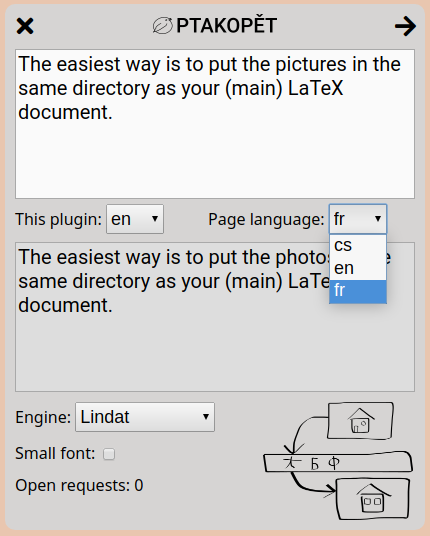
\includegraphics[width=0.35\textwidth]{screenshot_4}
\end{center}

\section{Possible extensions}
Future versions could also include a full fledged web interface similar to that of Google Translate (one page). Since Ptakopět is somewhat limited to backend capabilities, their extension is also desired (more language pairs, more information about translation confidence, etc.).

\section{Conclusion}
The first version of Ptakopět met all imposed usability criteria and didn't exceed the expected amount of work required. 

\end{document}
